\section{Introduction}
\subsection{Purpose}
This document defines the mission, goals and objectives, organization and responsibilities of the LSST Data Management Organization (DMO).  The document is currently scoped to define these elements for the LSST Design and Development, Construction, and Commissioning phases.  It does not presently address any ongoing mission for the DMO during LSST operations.

\subsection{Mission}
{\bf To be discussed in Tucson  - fundamentally do we not hav eto produce alerts/catalogues and images ? Not technology ...}
The mission of Data Management Organization (DMO) is to provide technology and operational capabilities for the acquisition, quality assessment, processing, end user and external system access, provenance, and archiving of open, publicly accessible, scientific data and associated engineering and quality data generated by the LSST as a result of scientific projects and telescope operations.

\subsection{Goals And Objectives}
The Data Management Organization will:
\begin{itemize}
\item Define the data products, data access mechanisms, and data management and curation requirements for the LSST
\item Assess current and LSST-timeframe technologies for use in providing engineered solutions to the requirements
\item Define the computing, communications, and storage infrastructure and services architecture underlying LSST data management
\item Select, implement, construct, test, document, and deploy the LSST data management infrastructure, middleware, applications, and external interfaces
\item Document the operational procedures associated with using and maintaining the LSST data management capabilities
\item Evaluate, select, recruit, hire/contract and direct permanent staff, contract, and in-kind resources in LSST and from partner organizations participating in LSST Data Management initiatives.

\end{itemize}
	


\section{Data Management Organization Structure}
This section defines the organization structure for the period in which the DM System is developed and commissioned, up to the start of LSST Observatory operations.  Refer to chapter 6 for Pre-Construction Phase Organization.
The DM Project Manager and DM Project Scientist, who are known collectively as DM Management, lead the DMO.  The Project Manager has direct responsibility for coordination with the overall LSST Project Office, the LSST Change Control Board, the LSST Corporation, and LSST partner organizations on all budgetary, schedule, and resource matters.  The Project Scientist has primary scientific and technical responsibility in the DMO and responsibility for ensuring that the scientific requirements of the LSST are supported, and is a member on the LSST Project Science Team (PST). 
As shown in \figref{fig:dmorg}, the organization now features lead institutions, each with responsibility for major element of the DM System (Level 2 Work Breakdown Structure elements).  For example, during Final Design, the Process Control and Archive Site Manager and Team at NCSA will be conducting prototyping activities in computing, data communications, and data storage to select and verify the ability of System technologies to support the LSST requirements.  They will also be involved in creating a supporting infrastructure for the DM Systems.  During Construction before the LSST first light time frame, these resources will be focused on implementation of the selected technologies.  In order to ensure that team functions as one integrated project, the institutions coordinate support by other lead institution team members directly through this organizational structure, as well as via a number of cross-organizational bodies (described later in this document). 
Also, due to the span of the organization, the DM Project Manager may be supported by one of the lead institution Project Managers as a Deputy Project Manager in these phases.

\begin{figure}[htbp]
\begin{center}
 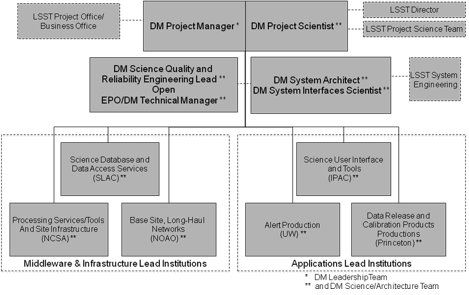
\includegraphics[width=0.9\textwidth]{images/dmorg}
\caption{Example Product tree a version of  CU1 product tree \label{fig:dmorg}}
\end{center}
\end{figure}

\section{Data Management Cross-Organizational Control Bodies}
Since the DM team is distributed in terms of geography and responsibility across the LSST partner and lead institutions, mechanisms are needed to ensure that the project remains on track at all times.  There are three primary coordinating bodies to ensure the management, technical, and quality integrity of the DM project.  All DM institutions have membership on these bodies, and all meet at least once per month during construction and commissioning.
\subsection{DM Leadership Team}

The DM Leadership Team (DMLT) purpose is to establish scope of work and resource allocation across DM and ensure overall project management integrity across DM.
The following mandate established the DMLT:

\begin{itemize}
\item Charter/purpose
\begin{itemize}
\item Establish scope of work and resource allocation across DM
\item Ensure overall project management integrity across DM
\item Ensure Earned Value management requirements are met
\end{itemize}
\item Membership
\begin{itemize}
\item Co-Chaired by the DM Project Manager, (TBD DM Deputy Project Manager(s)
\item Core members are Lead Institution Technical/Control Account Managers (T/CAMs or CAMs)
\end{itemize}
\item Responsibilities
\begin{itemize}
\item Prepares all budgets, schedules, plans
\item Meets every week to track progress, address issues/risks, adjust work assignments and schedules, and disseminate/discuss general PM communications
\item Creates and publishes monthly, quarterly, annual progress reports
\item Meets at start of each software development phase with SAT to establish detailed scope/work plan
\item Meets with SAT for change control (TCT)
\end{itemize}
\end{itemize}

The DM Leadership Team and the Science/Architecture Team (SAT) work in synchrony. The SAT (and the various DM team members as delegated) is responsible for creating, establishing, updating, analyzing, proposing the reference and DC designs and changes to them, whether they might affect the DMS requirements, the reference design, or the Data Challenges. The DMLT makes sure the requirements and architecture/design are estimated and scheduled in accordance with LSST Project required budgets and schedules.
\subsection{Science/ Architecture Team}

The Data Management Science/Architecture Team (SAT) is chaired by the Data Management System Architect and Project Scientist. The SAT is the DM-wide body that is charged with addressing issues of the overall requirements flowdown, architecture, and organization of the design of Data Management, both for the final LSST design and for the Data Challenges.

The designs and other high-level outputs of the SAT become part of the technical baselines for Data Management in the LSST project and for the Data Challenges. Approval and change control for these baselines are managed by the DM Technical Control Team (TCT).

\begin{itemize}
\item Charter/Purpose
\begin{itemize}
\item Support DM System Architect in ensuring that the DMS meets science requirements
\item Support DM Project Scientist in ensuring DMS has overall scientific integrity
\item Control all DMS internal and external interfaces
\item Perform or delegate due diligence for proposed technical baseline changes; then recommend changes (or no action) to the TCT
\item Decide issues involving internal, non-change-controlled DM architecture and design
\end{itemize}
\item Membership
\begin{itemize}
\item Co-Chaired by the DM System Architect (Kian-Tat Lim), DM Project Scientist (Mario Juric)
\item Core Members are Institutional Scientific/Technical Leads
\end{itemize}
\item Responsibilities
\begin{itemize}
\item Meets at start of each software development phase with DMLT to establish detailed scope/work plan
\item Meets with DMLT for change control (TCT)
\item Supports the System Architect's role in the systems engineering process, notably in the establishment and review of interface requirements and Interface Control Documents with the other LSST subsystems
\item Conducts (or delegates) design reviews and code reviews during the LSST development process
\item Endeavors to instill a productive and ethical engineering culture within DM
\item Commissions Working Groups
\begin{itemize}
\item Working groups are architectural (e.g. Applications, Middleware, Database, Infrastructure, Operations), span subsystems
\item Chaired by a member of the Science/Architecture Team
\item Members include other technical personnel, possibly including outside collaborators
\end{itemize}
\end{itemize}
\end{itemize}

\subsection{Technical Control Team}
The DM Technical Control Team has responsibility for issues similar to those of the LSST Configuration Control Board, but restricted to those contained within the DM subsystem. The TCT reviews and approves changes to all baselines in the LSST Data Management System, including proposed changes to the DM System Requirements' (DMSR), reference design, sizing model, i.e. any LDM-xxx baselined document.  The TCT makes sure these changes don't get into the baseline without proper change control.  Note that the TCT does not author the Technical Baseline and has no specific technical deliverable charter, but it does validate that the form and content of the Technical Baseline is consistent with LSST project standards such as the System Engineering Management Plan (SEMP).  Specific responsibilities for development of the Technical Baseline and evaluation of the content versus LSST and DM requirements are elsewhere in this document.
\begin{itemize}
\item Charter/purpose
\begin{itemize}
\item Ensure that the DM Technical Baseline (LDM-xxx) documents are baselined and once baselined only changed when necessary, according to LSST and DM configuration control processes
\end{itemize}
\item Membership
\begin{itemize}
\item Co-Chaired by the DM Project Manager and DM Project Scientist
\item Members include the DM System Architect, DM System Interfaces Scientist, DM SQuaRE Technical Manager
\item For on-line virtual meetings, if a quorum is not reached within one week, the DM Project Manager and the DM Project Scientist will make a unilateral decision
\end{itemize}
\item Responsibilities
\begin{itemize}
\item Determines when specification and deliverables are of sufficient maturity and quality to be baselined (placed under configuration controlled status) or released. The TCT reviews and approves proposed changes to baselined items.
\item Reviews and approves/rejects proposed changes to baselined items
\end{itemize}
\section{Data Management Problem Management/Escalation}
The above organizational structure allocates significant responsibility to lead institutions.  As such, when problems arise that cannot be solved with the responsibility and scope allocated to an institution, the path of escalation and resolution of such problems must be clear.  In cases of problems that cannot be solved within the DM organization, that escalation path must also be clear.  Figure depicts the escalation path for such problem resolution.


Figure 4 Problem Management/Escalation

Data Management Senior Positions and Responsibilities
LSST Data Management Managers and Staff
These individuals form the top level management of the DMO.
DM Project Manager
The DM Project Manager is responsible for the efficient coordination of all LSST activities and responsibilities assigned to the DMO. The DM Project Manager has the responsibility of establishing the organization, resources, and work assignments to provide DM solutions.  The DM Project Manager, serves as the DMO representative in the LSST Project Office and in that role is responsible for presenting DM initiative status and submitting new DM initiatives for approval consideration. Ultimately, the DM Project Manager, in conjunction with his / her peer Project Managers (Telescope, Camera), is responsible for delivering an integrated LSST system. The DM Project Manager reports to the LSST Project Manager. Specific responsibilities include:

\begin{itemize}
\item Manage the overall DM System
\item Define scope and funding for DM System 
\item Develop and implement the DM project management and control process, including earned value management
\item Approve the DM Work Breakdown Structure (WBS), budgets and resource estimates
\item Participate in identification of new DM partners 
\item Approve or execute as appropriate all DM outsourcing contracts 
\item Convene and/or participate in all DM reviews
\item Co-Chair the DM Leadership Team
\end{itemize}
DM Deputy Project Manager
The DM Deputy Project Manager, if this position is implemented, assists the DM Project Manager in the efficient coordination of all LSST activities and responsibilities assigned to the DMO.  Specific responsibilities are the same as the DM Project Manager, when delegated to the DM Deputy Project Manager by the DM Project Manager.
DM Project Scientist
The DM Project Scientist has ultimate responsibility for ensuring DMO initiatives provide solutions that meet the overall LSST scientific and technical requirements.  The DM Project Scientist must ensure correct specification of DM Scientific Requirements and proper translation of those requirements into derived information technology requirements and ultimately, into implemented solutions.  The DM Project Scientist must ensure that the DM subsystem is properly scoped and integrated within the overall LSST system.  The DM Project Scientist is also a member of the LSST Project Science Team (PST) and reports to the LSST Director. Specific responsibilities include:

\begin{itemize}
\item Responsible for the science deliverables of the DM System
\item Set requirements for the DMS that:
\end{itemize}
o Ensure that the design and operational flow of the data products meet the needs of the science community
o Ensure that the quality requirements of the data products will be / are being met by the DMS, with a particular emphasis on choice of appropriate application algorithms
\begin{itemize}
\item Set requirements for and assess/validate results of Data Challenges and other precursor experiments
\item Set requirements and assess/validate results for Data Releases
\item Convene and/or participate in all DM reviews
\item Co-Chair the DM Leadership Team and Science/Architecture Team
\end{itemize}
DM Science Quality and Reliability Engineering (SQuaRE) Leads
The DM SQuaRE Leads are the SQuaRE Lead Scientist and the SQuaRE Technical Manager.  The primary organizational responsibility for this Tucson-led group is to provide scientific and technical feedback to the LSST DM Manager that demonstrates LSST/AURA DM is fulfilling its responsibilities as charged by the NSF with regards to science quality and software/IT performance and reliability.
They are responsible for monitoring the reliability and maintainability of software developed by DM and the quality of the data products produced by the DM software in production. SQuaRE's activities span processes and environments for software development, integration test and distribution.  SQuaRE also assumes responsibility for delivering any work in this area, though in many cases this may involve effort across the DM team. 
As such, areas of activity include:
\begin{itemize}
\item Development of algorithms to detect and analyze quality issues with data
\item Infrastructure development to support the generation, collection, and analysis of data quality and performance metrics
\item DM developer support services to ensure DM is using appropriate tools to aid software quality
\item Support of publicly released software products, including porting and distributing it according to the scientific community?s needs.
\end{itemize}

In the event that SQuaRE identifies issues with the performance or future maintainability of the DM codebase, it brings them to the attention of the DM System Architect, who is ultimately responsible to decide who will address them and how. In the event that SQuaRE identifies issues with the quality of the data, it brings them to the attention of the DM Project Scientist. 
DM System Architect
The DM System Architect is responsible for ensuring that all elements of the DM systems, including infrastructure, middleware, applications, and interfaces, adhere to a documented, integrated architecture, consistent with the overall LSST systems architecture.  The DM System Architect reports to the DM Project Manager and DM Project Scientist. Specific responsibilities include:
\begin{itemize}
\item Responsible for the overall design integrity of the DMS as a system, including
\end{itemize}
o Internal and external interfaces and overall architecture
o Use of frameworks and off-the-shelf components
o Sound engineering practice
\begin{itemize}
\item Ensure that the DMS design is traceable to an meets the requirements set by the DM Project Scientist, through requirements/design models and technical reviews
\item Set standards for development, implementation, and documentation of the DMS, and ensure that they are being met by all DM participants
\item Participate in stakeholder and end user coordination and approval processes and reviews
\item Member of the LSST System Engineering Team
\item Co-chair the DM Science/Architecture Team
\end{itemize}


Lead Institution Senior Positions
Each Lead Institution has a Project Manager and Scientific/Engineering Lead, who jointly have overall end product responsibility for a broad area of DM work, typically a Work Breakdown Structure (WBS) Level 2 element. They are supervisors of the team at that institution.  Their roles and responsibilities are similar to the DM Project Manager, DM Project Scientist, and DM System Architect, and DM QA and Test Lead, but within the scope of work assigned to that institution.  These leaders are bound to acknowledge and implement direction from the DM leadership in all matters pertaining to the DM project.  The DM Project Manager and DM Project Scientist have direct input into the performance appraisals of the Institution Project Manager and Scientific/Engineering Lead. 

Appendix A DMO Discussion and Decision Making Process

The Escalation process only occurs when the issue cannot be resolved within the DMO, i.e. when the following internal discussion and decision making process has failed to yield a decision.
Empowerment
All DMO team members are empowered by the DM Project Manager (PM) and Project Scientist (PS) to make decisions on any DM-internal matter, including technical/algorithm issues, process improvements, tool choices, etc., when:
A) they are willing and able to do the work to implement the decision or with people who agree with the team memaber,
B) they (collectively) are willing and able to fix any problems if it goes wrong, and
C) they believe that all affected parties (including your immediate manager) would not seriously object to your decision and implementation.
RFC Process
If the above three criteria are not met, perhaps because the team member doesn't know all the affected parties or because they don't know their positions, the team member should publish the proposed decision and implementation as a JIRA issue in the Request For Comments (RFC) project with a component of "DM".

It is usually difficult to determine all the affected parties for published package interfaces. Changes to interfaces should thus typically go through this process.

It's a good idea to contact any known affected parties before starting this process to check that the resolution is sensible. The institutional technical manager is always affected, as she or he is responsible for tracking the work schedule. If work for others is being proposed, they are obviously affected. The institutional scientist, the DM System Architect (SA), the DM Interface Scientist (IS), and the DM Project Scientist (PS) are also valuable resources for determining affected parties.

The purpose of an RFC is to inform others about the existence and content of the proposed decision and implementation in order to allow them to evaluate its impact, comment on it, refine it if necessary, and agree (implicitly or explicitly) or object (explicitly) to its execution.

The discussion of the RFC takes place in the medium of the requestor's choosing (e.g., a specific mailing list, the RFC JIRA issue itself, a HipChat room, a convened videocon, some combination of those, etc.), but the requestor should be open to private communications as well.

In the RFC process, the opinions of those who will be doing the work (and fixing any problems if something goes wrong) are given more weight. In some cases, this may mean that the RFC issue's Assignee passes to someone else. The opinions of more senior people or people more experienced in the area should also be given more weight and may also result in the Assignee changing.

The Assignee is responsible for determining when no serious objections remain.  In particular, there is no need to call for a formal vote on the (refined) resolution. If no explicit objections have been raised within, typically, 72 hours for "ordinary" issues and 1 week for "major" issues, the Assignee should assume that there are none. This is known as "lazy consensus". When this state has been reached, the Assignee is responsible for ensuring that the final consensus has been recorded in the RFC issue before closing it and proceeding with implementation of the decision.

The requestor must be especially careful about not making irreversible changes in the "lazy consensus" time period unless they are absolutely certain there's a general agreement on the stated course of action. If something is broken, the requestor must be be ready to fix it. It is critical to apply sound reasoning and good judgement about what may be acceptable and what might be not. Mistakes will happen; accept that occasionally there will be a requirement to revert an action for which it was thought agreement existed.
Exceptions and Appeals
Some proposed resolutions may require changes to one or more of the baselined, change-controlled documents describing the Data Management system (those in DocuShare with an LDM- handle or marked as change-controlled in Confluence).  Note that major changes to budget or scope will almost certainly affect one or more LDM- documents.  In this case only, the DM Technical Control Team (TCT), consisting of the DM PM, PS, SA, and IS, may empanel an ad hoc committee including the lead author of the document and other relevant experts. This committee or the TCT itself must *explicitly* approve the change.

Change-controlled documents with other handles, such as LSE- or LPM-, including inter-subsystem interfaces, have project-wide change control processes. Please consult the DM PM, SA, or IS for more information.
At least one member of the DM TCT will read each RFC to determine if it might affect a change-controlled document.

If the DMO team can't converge on a resolution to an RFC that has no serious objections but the requestor still feel that something must be done, the request will be escalated. In most non-trivial cases, they will, with the advice of the SA, empanel a group of experts to which they will delegate the right to make the decision, by voting if need be.

Formalities
For project management purposes, RFCs are formally proposals made to the DM PM and PS who by default are responsible for everything in DM (they "own" all problems). As owners, they have the final word in accepting or rejecting all proposals. Functionally, they delegate that ownership ? the right and responsibility to make decisions -- to others within the team (e.g. the SA, IS, group leads, etc.) who are expected to delegate it even further. Notifying the institutional technical manager about an RFC serves to inform the DM PM.

Appendix B Pre-Construction Phase Organization
This section is historical in nature and describes the DM Organization as it has evolved during the Conceptual, Preliminary, and Final Design Phases prior to Construction.
Conceptual Design Phase
As shown in Figure 1, during the Conceptual Design Phase, the Project Manager and Project Scientist jointly supervise several Working Group, which are aligned by functional area.  The Working Group Leads are strictly technical leaders responsible for specific work areas, and have no budgetary or schedule authority.  Their primary work is the development of requirements and architecture in each of these functional areas.

\end{enumerate}

\section{LSST Science Council no longer exists. It has been replaced by the LSST Project Science Team and the LSST Science Advisory Committee
 \label{sect:LSSTScienceCouncilnolongerexists.IthasbeenreplacedbytheLSSTProjectScienceTeamandtheLSSTScienceAdvisoryCommittee
}}
Figure 5 Data Management Conceptual Design Phase Organization


Preliminary Design Phase
The organization transitions to a more complex structure during Preliminary Design, as the role of each DM partner institution is solidified, and D\&D prototype development projects called Data Challenges become a primary organizing/tasking vehicle for D\&D work.  The Working Groups still remain and play a cross-institutional functional role in each area, but there is a more formal structure for work allocation and responsibility, as shown in Figure 2.


\section{LSST Science Council no longer exists. It has been replaced by the LSST Project Science Team and the LSST Science Advisory Committee
 \label{sect:LSSTScienceCouncilnolongerexists.IthasbeenreplacedbytheLSSTProjectScienceTeamandtheLSSTScienceAdvisoryCommittee
}}

Figure 6 Data Management Preliminary Design Phase Organization

In this phase, new positions reporting to the Project Manager and Project Scientist are added.  First, there is the DM System QA and Test Lead, who assists the Project Manager in preparation of formal plans, processes, and environments for software development, integration, and test. 
A Data Management System Architect supports the Project Manager and Project Scientist in matters related to LSST system engineering, including other subsystem interfaces, overall LSST system control, real-time external system interfaces (e.g. alerting), simulation, and end-to-end system engineering for quality assessment.
Finally, temporary Data Challenge Teams consisting of astronomers and engineers are formed for prototyping specific critical design aspects that have high risk (e.g. precursor and simulated data processing and prototype work, research and development of new algorithms for moving object detection or data distribution).  Each Data Challenge Team has a designated Project Manager who reports to the Project Manager and Scientist who reports to the Project Scientist for the duration of the Data Challenge.


Final Design Phase
During Final Design Phase, the organization structure transitions to one that will persist for the remainder of the period in which the DM System is developed and commissioned, up to the start of LSST Observatory operations.
As shown in Figure 3, the organization now features lead institutions, each with responsibility for major element of the DM System (Level 2 Work Breakdown Structure elements) and Project Manager.  For example, during Final Design, the Processing Services/Tools and Archive Site Manager and Team at NCSA will be conducting prototyping activities in computing, data communications, and data storage to select and verify the ability of System technologies to support the LSST requirements.  They will also be involved in creating a supporting infrastructure for the DM Systems.  During Construction before the LSST first light time frame, these resources will be focused on implementation of the selected technologies.  In order to ensure that team functions as one integrated project, the institutions coordinate support by other lead institution team members directly through this organizational structure, as well as via a number of cross-organizational bodies (described later in this document). 
Also, due to the span of the organization, the DM Project Manager will be supported by one of the lead institution Project Managers as a Deputy Project Manager in these phases.


Figure 7 Data Management Final Design Phase Organization





?LSST Corporation, 2016
Page 1 of 15


